%sazeno v XeLaTeX, aby slo pismo TImes New Roman 
%nasledujici nastaveni dle BP "Sablony odbornych praci pro LaTeX"
\documentclass[12pt, twoside]{book} % vel. pisma, oboustr. tisk a typ dokumentu
\usepackage[utf8]{inputenc} % kodovani
\usepackage{cite} % citovani
\usepackage[IL2]{fontenc}
\usepackage{textgreek}
\usepackage[czech]{babel}
\usepackage{tabularx}
\usepackage[bf,sf]{titlesec}
\usepackage[top=2.5cm, bottom=2.5cm, left=3.5cm, right=2.5cm, includefoot]{geometry}
\usepackage[hidelinks]{hyperref}
\usepackage{indentfirst}
\setlength{\parindent}{10mm}
\usepackage{color}
\addto\captionsczech{
  \renewcommand{\contentsname}%
    {Contents}%
}
%%%%%%%%%%%%%%%%%%%%%%%%%%%%%%%%%%%%%%

%nasledujici baliky az po begin{document} jsou z prednastaveni sablony pro texworks
%\usepackage{geometry} % rozmery stran
%\geometry{a4paper} % or letterpaper (US) or a5paper or....
% \geometry{margin=2in} % for example, change the margins to 2 inches all round
% \geometry{landscape} % set up the page for landscape
%   read geometry.pdf for detailed page layout information
% \usepackage[parfill]{parskip} % Activate to begin paragraphs with an empty line rather than an indent
\usepackage{graphicx} % support the \includegraphics command and options
\usepackage{booktabs} % for much better looking tables
\usepackage{array} % for better arrays (eg matrices) in maths
\usepackage{paralist} % very flexible & customisable lists (eg. enumerate/itemize, etc.)
\usepackage{verbatim} % adds environment for commenting out blocks of text & for better verbatim
\usepackage{subfig} % make it possible to include more than one captioned figure/table in a single float
\usepackage{fontspec}
\usepackage[counterclockwise, figuresright]{rotating}
\usepackage{tikz}

\usepackage{floatrow}
\floatsetup[table]{capposition=top}
\floatsetup[figure]{capposition=top}

\usepackage{caption}
\captionsetup[table]{name=Table}
\captionsetup[figure]{name=Figure}

\setmainfont{Times New Roman}

%%% HEADERS & FOOTERS
\usepackage{fancyhdr} % This should be set AFTER setting up the page geometry
\pagestyle{fancy} % options: empty , plain , fancy
\renewcommand{\headrulewidth}{0pt} % customise the layout...
\lhead{}\chead{}\rhead{}
\lfoot{}\cfoot{\thepage}\rfoot{}

\addto\captionsczech{\renewcommand{\chaptername}{Chapter}}

%%% SECTION TITLE APPEARANCE
\usepackage{sectsty}
%\allsectionsfont{\sffamily\mdseries\upshape} % (See the fntguide.pdf for font help)
% (This matches ConTeXt defaults)

%%% ToC (table of contents) APPEARANCE
\usepackage[nottoc,notlof,notlot]{tocbibind} % Put the bibliography in the ToC
\usepackage[titles,subfigure]{tocloft} % Alter the style of the Table of Contents
\renewcommand{\cftsecfont}{\rmfamily\mdseries\upshape}
\renewcommand{\cftsecpagefont}{\rmfamily\mdseries\upshape} % No bold!
\renewcommand{\baselinestretch}{1.5}
%%%%%%%%%%%%%%%%%%%%%%%%%%%%%%%%%%%%%%%%%%%

\begin{document}

\begin{titlepage}   %titulni strana
\centering
\begin{center}
\textsc{ Vysoká škola ekonomická v Praze}\\[20pt]
\textbf{Národohospodářská fakulta}\\[20pt]
\textsc{Hlavní specializace: Ekonomická analýza}\\[14pt]

\begin{figure}[h]
  \centering
  
\includegraphics{obr1_nf_logo}
\end{figure}

\textsc{Are judges good at estimating the future? An application of machine learning on custody decision}\\[24pt]
\textit{diplomová práce}\\[19pt]
\vspace*{\fill}

\begin{flushleft}
\textbf{Autor: Jakub Panýr}\\[17pt] 
\textbf{Vedoucí práce:  Ing. Jan Vávra}\\[17pt]  
\textbf{Rok: 2018}\\[17pt] 
\end{flushleft}

\end{center}
\end{titlepage}

\pagestyle{empty}     %volna strana bez cislovani
\clearpage\mbox{}\clearpage


\section*{Declaration}      %prohlaseni v aj a cj
\noindent
I declare that this thesis and the work presented in it are my own and I used only sources mentioned in the References section.

\section*{Prohlášení}
\noindent 
Prohlašuji na svou čest, že jsem diplomovou práci vypracoval samostatně a s použitím 
uvedené literatury.

\vspace*{\fill}
\noindent
V Jablonci nad Nisou dne \today \hfill \dotfill

\begin{minipage}{\textwidth}
\hfill Jakub Panýr \hspace*{2.5cm}
\end{minipage} \newpage

\section*{Acknowledgment}        %podekovani v aj
\noindent I am very thankful to all people who have helped me, especially to my advisor Jan Vávra. \newpage

\section*{Assignment}           %zadani v aj
Aim of this diploma thesis is to analyze the efficiency of a pretrial custody in the Czech Republic using machine learning.\newline
Currently, there are more than 1,700 accused awaiting for trial in the Czech prisons. Taking the person into custody brings costs of imprisonment to the state and opportunity cost of social and work development to the individual. This costs should be justified by eliminating the risk of nonappearance to trial, escape or continuation in the criminal activity. Aim of this thesis is to shed light on the efficiency of the custody process represented by trade-off above and the decision making of the judges. Possible improvement of custody decision may reduce jailing rates with no change in rate of crime (or reduce crime rate with no change in jailing rate). \newline
In the theoretical part of the thesis, I will summarize the literature of judicial behavior with an accent to on custody decision. Part will conclude with a short exposition of current use of machine learning techniques in economics and their application on economics of crime. \newline
Practical part of the thesis will start by presenting summary statistics about the development and usage of the custody in the Czech Republic. Then I will closely follow the methodology used in (Kleinberg, Jon, et al. 2018), adapted to Czech context. For prediction of the custody decision and probability of re-offending or avoiding the trial, machine learning models will be formulated and selected based on predictive performance from a wide array of possible techniques. Models will be trained on micro data about custody decisions from the Czech Republic criminal system. Results from the models will be interpreted to reveal factors behind pretrial custody decision and quasi-experimental design exploiting differences between districts will be used to estimate over-usage or under-usage of custody. \newpage

\section*{Abstract}   %abstrakt v aj a nasledne v cj
\textbf{Keywords:} \newline
\textbf{JEL Classification:}


\section*{Abstrakt}
\textbf{Klíčová slova:} \newline
\textbf{JEL Klasifikace:}

\tableofcontents    %obsah
\renewcommand{\thepage}{\arabic{page}}
\renewcommand{\baselinestretch}{1.5}
\addtocontents{toc}{\protect\thispagestyle{empty}}


\chapter*{Introduction}     %uvod
\addcontentsline{toc}{chapter}{Introduction}
\pagestyle{plain}
Introduction text.


\chapter{Theoretical part}    %teoreticka cast
This section offers firstly a brief review of the literature in the field of economics of crime and advances in that field relevant to my thesis. Then I introduce machine learning as a tool (or a group of tools) of a potential usage for economists. After that I am dealing with a custody decision as a special case of economics of crime problem that may be solved, at least partially, using machine learning techniques.\newline
After review of the literature I present a theory behind those techniques I am using, with regard to the fact that they are not a standard part of a curriculum of economic analysis program at University of Economics Prague. Finally some assumptions together with a theoretical model are formulated. 

\section{Literature review}     %popis literatury k tematu
The economics of crime is a rich area of economic science that have started its modern era probably with a publication of an influential paper by Gary Becker (Becker, 1968). However his attention was more focused towards microeconomic foundations of a crime decision of potential criminals as well as towards optimal level of crime in some society (given that an enforcement of a law is an activity that brings costs to the society and because of that optimal level of crime could be different from zero). Heckmann (2015) supports this idea of Becker as an inventor of the economics of crime and offers further informations on his role in the development of this branch.\newline
Nonetheless my attention is rather focused on so-called prediction policy problems in the area of the economics of crime. Because a prediction forms a substantial portion of a policy decision, I will focus mostly on the literature relevant to problems connected with a policy prediction. As Kleinberg et al. (2018) assert, a question of improving decision making with an aid of statistically-driven prediction is not a completely new. They point to research from psychology (Meehl, 1954, who focused on a comparison of clinical and statistical methods in predictions) and criminology (Ohlin and Duncan, 1949, who were trying to compare results of various then known prediction techniques). \newline
More interestingly Kleinberg et al. (2018) refer to the fact that relevance of policy prediction problems has increased from the era of 1950's given two important facts. Firstly, very large volumes of data (nowadays often called “Big data”) are now available and offer an opportunity to more fruitfully gather informations, as, \textit{ceteris paribus}, greater dataset is better in the sense of a bigger possibility of obtaining more informations about data. Secondly, and to my opinion more importantly, we have been witnesses of an emergence and a consequent development of new statistical (or more generally mathematical) techniques for dealing with data. Not only those new techniques were mathematically and rigorously formulated (as in, say, Friedman, 2001) but they can also exploit an advancement in the area of computers in general. This could mean for example an usage of parallel computing as CUDA platform and so on. In general, subarea of an artificial intelligence that concerns with a study of possible improvement of mathematical models and algorithms used by computers for performing some specific task (as a classification, prediction, clustering, \ldots) is called the Machine Learning (from now I will use, when it is useful, ML as an abbreviation). ML can be also understood ‘as a set of methods that can automatically detect patterns in data, and then use uncovered patterns to predict future data, or to perform other kinds of decision making under uncertainty (such as planning how to collect more data!)’ (Murphy, 2012, who offers a systematical introduction to ML adopting a probabilistic approach). Another introduction to ML, though more brief one that Murphy (2012), is an article by Hal Varian (2014), which is aimed especially on economists. Mullainathan and Spiess (2017) discuss machine learning from the econometrician's point of a view and finally Einav and Levin (2014) complement introductory articles on ML with a study of an influence of so-called big data era on an economic science. \newline
At this moment I could finally concentrate on the connecting of these two areas — economics-of-crime policy predictions problems and a machine learning. A framework for this connection is provided by an existence of a special case of the judge's decision, i.e. by a decision about imposing a custody. This kind of decision offers an ideal opportunity to find out the value of machine learning techniques in a policy prediction problems. As Kleinberg et al. (2018) write, it is, among other things, caused by an unique nature of a custody decision, especially by a concreteness of a prediction task and (usually) large volume of available data. Ideally, judge should base her prediction on a processing of available informations as a current offense and circumstances of that offense (if it was a violent crime, if there were money involved and so on) and on an evaluation of these informations with regard to the fact that she is confronted by a trade-off. The trade-off is present mostly because of the presence of costs of an incarceration. If it were cost-free, then ideal solution (decision) for a judge would be an imprisonment of all people, just because of the fact that an imprisonment reduces crime rate almost automatically. However the fact is that an incarceration has costs associated and for that she has to find a balance between an imprisonment of a person (which leads to the reduction in the crime rate, or at least to the absence of an increase in the crime rate, \textit{ceteris paribus}, and at the same time to the increase of total society costs from an imprisonment) and between releasing of a person (that obviously brings no costs of an incarceration, but it may leads to an increase in the crime rate). This prediction could be easily made by some algorithm (be it called machine learning algorithm or not) in the similar manner to the use of an algorithm to, say, prediction of time series, e-mail spam detection or recognizing the object on an image. My concern is to discuss possible benefits and costs of using that kind of a prediction. Of course that prediction is not meant to be used solely, but rather as a companion tool for judges, who could just enter informations about a suspect person into computer and then combine their judgment with a result of an algorithm. \newline
I closely follow a methodology of Kleinberg et al. (2018), who are dealing with the same problem in the context of the United States. As they say, a problematic challenge ‘is not so much in building the algorithm, but rather in assesing whether its predictions actually improve on judges' decisions’ (\textit{ibidem}). Problematic is mostly the fact that we are missing a counterfactual in the sense that we do not know if jailed defendants would have comitted crime after they had been relased by a judge. It is similar to the problem in credit risk area, where for example single mothers are not usually given a loan and we do not know whether they would have repaid their loans or not (of course when they are not given a loan, there is no problem with an absence of payments, however it in a certain way disadvantages these single mothers). Nevertheless one can overcome that problem by its one-sideness. As I have mentioned with an example of single mothers asking for a loan, one can easily evaluate the counterfactual in the case that algorithm jail some additional  defendant. Then we know that jailing these defendants reduces crime rate (or better say it will ensure that crime rate of these people will be equal to zero) similarly to our certainty that not giving a loan will ensure zero rate of non-payment. So there remains an issue with the situation when an algorithm release defendant who was originally not released by a judge. This problem is sometimes called “a missing-label problem”. Apart from Kleinberg et al. (2018) it is solved for example by Kling (2006) who has used differences in judge's leniency for an estimation of effects of an incarceration on subsequent labor market outcomes of jailed individuals or by Di Tella and Schargrodsky (2013) in their study of recidivism in Argentina, who again use differences in judge's leniency (in their case different judge's leniency is projected into different rate of electronic monitoring for an otherwise similar population). This procedure (known as a contraction) benefits from the fact that we can combine a result from an algorithm with a judgment of a lenient group of judges and compare that result with a judgment of a more strict group. As mentioned in Kleinberg et al. (2018), we can then compare these results without assuming specific preferences of a society. In other words we do not have to assume specific preferences (e.g. that society tolerates crime rate of, say, n \% given release rate of m \%) and we can just contrast results of lenient judge who uses an aid of an algorithm with results of stricter judge and observe whether there is a possibility to increase release rate while maintaining crime rates, or a possibility to decrease crime rate while maintaining release rate. Both cases are then understood as an improvement.\newline
Results of Kleinberg et al. (2018) suggest that there may exist such an algorithm, at least for the case of New York City (although they have proved that their algorithm is sufficiently robust). One of their simulations show that their algorithm is able to help the judges because, irrespectively of judge's preferences, application of the results leads up to the 24.7\% reduction in the crime rate (with no change in jailing rate) or up to 41.9\% reduction in jailing rate (with no change in crime rate). Another study is Lakkaraju et al. (2017) who also address the problem with selective labels (situation when we are missing labels as a result of a choice of human decision-maker, be it a judge deciding about imposing of a custody or a doctor predicting probability of a neurological recovery of a patient in coma, hence deciding whether they should continue in the life support of a patient. Their results suggest that a contraction procedure is capable of solving the problem and that it can be ‘readily applied to various domains where human decision making is involved ranging from public policy to health care and education’ (\textit{ibidem}). \newline 
In the next subsection \ref{1.2} I introduce a theoretical models later empirically tested to the verification of a null hypothesis that there exists an algorithm that may improve a custody decision in the sense that its use leads \textit{primo} to the reduction of crime rate with no change in jailing rate or \textit{secundo} to the reduction of jailing rate with no change in crime rate. 




\section{Theoretical models}    %formulace teoretickych veci
 \label{1.2}
Dodelat tuto sekci - formulovat teoreticky modely.
\medskip
\newline
In this section I present a simple theoretical model used as an empirical strategy to solve a custody decision problem and overcome difficulties associated with it. In the second chapter I empirically test my model using micro data from Czech judicial (or rather say criminal) system. I will build an algorithm which is in fact a case of a gradient boosted decision trees algorithm (Friedman 2001). This algorithm is based on an idea of a decision tree that is summarized in the caption of Figure 1.1 (basically one has a graph with a tree-like structure, where every node involves  some decision, e.g. whether person is male or female or whether that person has comitted crime before, is made and at final nodes one obtain prediction or classification of that specific case.\newline
Problem with such a tree is that only tree cannot do such a good job at classifying or predicting as a collection of trees somehow combined together. Becasue of that fact, ensembling techniques, which are techniques that combine multiple hypotheses to perform with an aim of performing better than a just one hypothesis (specifically to our case with an aim of performing better than just a one decision tree), were developed.\footnote{For more information on this confront Berk (2012) or Hastie, Tibshirani and Friedman (2009).} They can be divided into two groups, bagging ensembles and boosting ensembles, when example of bagging ensemble is a random forest (each tree is train independently and these trees are then combined into, unsurprisingly, forest) and example of a boosting ensemble is a gradient boosting machine, which is ensemble I am using. Figure 1.2 offers a schematical representation of the way how it works together with a commentary. 







\begin{figure}[H]
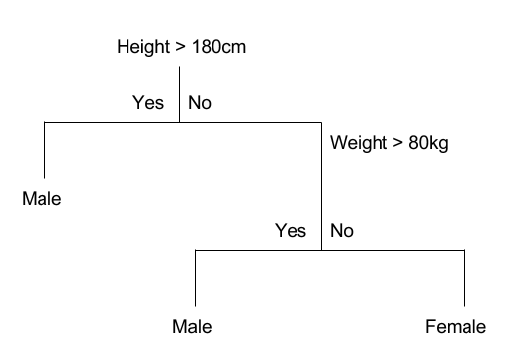
\includegraphics[width=\textwidth]{decisiontree.png}
\captionof{figure}{Example of a decision tree}
\label{Figure 1.1}
{\small Source: \url{https://machinelearningmastery.com/classification-and-regression-trees-for-machine-learning/} \newline
This figure shows an elementary decision tree classifier for decision whether sex of a given person is male or female. As reader can see, that decision is based on values of two variables, height and weight, when first node (root node) splits cases accordingly to the height of a person – if some person is higher than 180 cm, classifier assigns label (terminal node) “Male” to that person. Next node (decision node) splits observations of people with height lower or equal to 180 cm with respect to the weight of that person. Clearly one who has 170 cm and 65 kg is classified, or labeled, as a woman.}
\end{figure}


\begin{figure}[H]
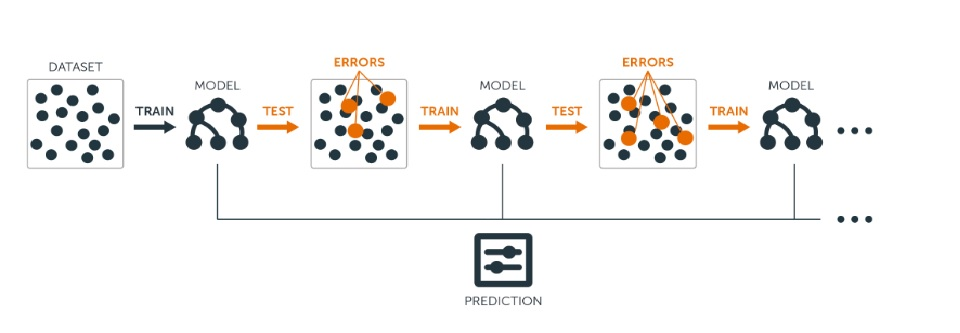
\includegraphics[width=\textwidth]{boosting_scheme.jpg}
\captionof{figure}{Scheme of a boosting of a decision tree}
{\small Source: \url{https://www.datacamp.com/community/tutorials/decision-trees-R} \newline
At this figure reader can find schematical representation of a boosting of decision tree. Basically prediction is made by a sequential modification of original decision tree in a greedy fashion, i.e. by a modification that at first tries to correct tree with respect to the worst predictions and to some loss function. It is called greedy because correcting of those worst predictions is in a certain way the simplest (the greediest) way to improve overall predictive ability. It is analogical to a simplicity of finding the spanning tree in a graph by a greedy algorithm, when one starts with two nodes connected by a shortest edge (i.e. a edge with a lowest weight attached to it) and then just add another edges, until he chooses all edges, while avoiding a circularization of a graph. }
\end{figure}




\chapter{Practical part}        %prakticka cast
\label{2}



This chapter provides an empirical analysis of the main research question, i.e. if there exists an algorithm that could be helpful for decision of judges on imposing of a custody. At first, I will describe schematically how custody decision works in the Czech Republic. By that I mean description of phases of the process in the Czech legal system. Also I will offer basic statistics of those phases for years 2008-2017, i.e. for years my dataset is coming from. After that follow summary statistics of my dataset together with a brief commentary.\newline
Biggest part of the chapter is then an empirical model itself. Firstly I present results of a model that tries to explain custody decision and its comparison with logistic regression. In the next subchapter I present results of a second model that has crime as a output and results of contraction (procedure for dealing with missing counterfactual). These results are used to answer main research question. After that I am looking for a possible explanation of the fact that judges may be making a mistake while deciding on a custody, which could be not a such mistake when I take into account possibility of a existence of different production function of the judges from that function defined by me. Lastly tests for a robustness of my model and tests for possible human data mining (which is what researcher should try to avoid) are conducted. 


\section{Custody in the Czech Republic}      %popisne statistiky vazby v poslednich letech s komentarem

Na toto misto doplnit popisny komentar ke grafu a tabulce; dale zdroje a zpracovani priloh a rovnez info o 
vazbe v Cr, mysleno "jak to u nas funguje" (neco se stane -> policie -> sz -> soudce -> vazba) plus odkaz na prislusne paragrafy, resp. i napriklad na vezenske rocenky ci na tu rigorozni praci. 


\begin{figure}[H]
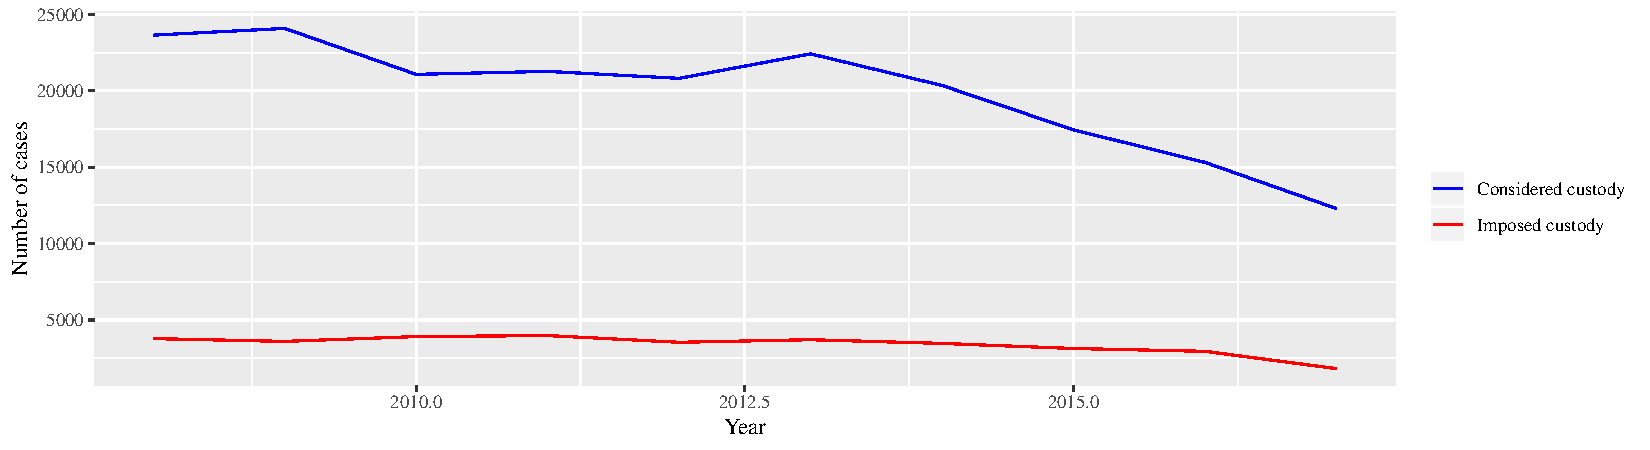
\includegraphics[width=\textwidth]{plot_21_1.pdf}
\captionof{figure}{Time evolution of number of cases handled over to a judge and of custody imposed}
{\small Source: }
\end{figure}

\newpage

\begin{sidewaystable}[H]
\centering
\begin{tabular}{rrrrrrrr}
  \hline
 Year & Possible Custody (PC) & Public Prosecution (PP) & Custody (C) & Average Length of Custody & C/PC & PC/PP \\ 
  \hline
 2008 & 23651 & 108439 & 3774 & 3.59 & 0.16 & 0.22 \\ 
   2009 & 24091 & 108599 & 3591 & 3.59 & 0.15 & 0.22 \\ 
   2010 & 21082 & 100946 & 3906 & 3.75 & 0.19 & 0.21 \\ 
   2011 & 21276 & 103624 & 3973 & 3.75 & 0.19 & 0.21 \\ 
  2012 & 20821 & 102061 & 3533 & 3.91 & 0.17 & 0.20 \\ 
   2013 & 22426 & 106507 & 3702 & 3.80 & 0.17 & 0.21 \\ 
   2014 & 20357 & 103099 & 3459 & 3.92 & 0.17 & 0.20 \\ 
   2015 & 17448 & 91357 & 3126 & 3.85 & 0.18 & 0.19 \\ 
  2016 & 15319 & 83222 & 2942 & 3.99 & 0.19 & 0.18 \\ 
   2017 & 12294 & 65184 & 1807 & 3.26 & 0.15 & 0.19 \\ 
   \hline
\end{tabular}
  \caption{Overall statistics of Custody in the Czech Republic for years 2008 to 2017 }

 \medskip
{\small This table provides basic statistics of custody in the Czech Republic between years 2008 and 2017. Every row represents one year (captured in first column). In second column is total number of Possible Custody (PC), that is a number of cases that state prosecutor handed over to a judge, third column represents total number of cases received by Public Prosecution (PP), ratio of these two numbers (share of cases handed over from prosecutor to a judge) is then in last column. Fourth column is a total number of imposed custody for a given year, sixth column agains captures ratio, now share of custody on number of cases received by a judge. Finally in fifth column reader can find information about average length of custody in months.}
\end{sidewaystable}













\section{Data}     %popisne statistiky uzitych dat s komentarem

Nejprve popis datasetu jakozto jaky je jeho zdroj atd... dale info o vycisteni a  rozdeleni na (train, test, imputation, holdout) a proc se to dela (prilozit schematicky obrazek podobny tomu v clanku Kleinberga). Dale popisne statistiky (workout setu, tj. bez holdout) s komentarem. Rovnez rozdeleni popis. stat. na ty propustene (ve smyslu vazby) a nepropustene a komentar k tomuto (zda se nejak lisi tyto dve skupiny) -  pres t-test shodnosti prumeru. Tabulka nize bude "dodelana". 

\begin{table}[ht]
\centering
\begin{tabular}{rlll}
  \hline
 & Name of dataset & Number of observations & Relative frequency \\ 
  \hline
 & Full dataset & 98666 & 1 \\ 
  & Hold-out sample & 9866 & 0.1 \\ 
   & Workout set & 88800 & 0.9 \\ 
   & 	\hspace{1cm}Training set & 35520 & 0.36 \\ 
  & 	\hspace{1cm}Test set & 35520 & 0.36 \\ 
   &	\hspace{1cm}Imputation set & 17760 & 0.18 \\ 
   \hline
\end{tabular}

\caption{Partition of full dataset}
\medskip
{\small This table provides information on the partitioning of original dataset (i.e. "full workout set"). I am reminding that firstly I had decomposed original dataset into hold-out sample (sometimes called "true hold-out set") and workout set. Then I made further partitioning of workout set into three sets - training set, test set and imputation set. Second column gives total numbers of observations in a set. Besides of that, relative frequencies in third column refer to relative frequencies of number of observations in a given set to the total number of observations. }

\end{table}


\begin{table}[H]
\centering
\begin{tabular}{rrrrr}
  \hline
Variable & Full sample & Released by judge & Detained by judge & P-value \\ 
  \hline
custody & 0.14 & 0.00 & 1.00 & 0.00 \\ 
  reoff & 0.06 & 0.07 & 0.00 & 0.00 \\ 
  viol & 0.11 & 0.12 & 0.00 & 0.00 \\ 
  nonenter & 0.05 & 0.05 & 0.00 & 0.00 \\ 
  dmy\_vodsouz & 0.92 & 0.92 & 0.94 & 0.00 \\ 
  dmy\_tr\_nepo & 0.31 & 0.24 & 0.74 & 0.00 \\ 
  dmy\_tr\_po & 0.45 & 0.49 & 0.18 & 0.00 \\ 
  vek & 32.98 & 33.00 & 32.91 & 0.37 \\ 
  dmy\_cizinec & 0.14 & 0.14 & 0.15 & 0.01 \\ 
  dmy\_zena & 0.11 & 0.12 & 0.06 & 0.00 \\ 
  dmy\_vzd\_bez & 0.03 & 0.03 & 0.04 & 0.00 \\ 
  dmy\_vzd\_zakl & 0.78 & 0.78 & 0.82 & 0.00 \\ 
  dmy\_vzd\_str & 0.16 & 0.16 & 0.13 & 0.00 \\ 
  dmy\_vzd\_vys & 0.02 & 0.02 & 0.01 & 0.00 \\ 
  dmy\_recidivist & 0.10 & 0.09 & 0.13 & 0.00 \\ 
  dmy\_prv & 0.26 & 0.27 & 0.20 & 0.00 \\ 
  oca1 & 0.01 & 0.00 & 0.05 & 0.00 \\ 
  oca2 & 0.06 & 0.03 & 0.21 & 0.00 \\ 
  oca3 & 0.37 & 0.40 & 0.24 & 0.00 \\ 
  oca4 & 0.03 & 0.03 & 0.04 & 0.00 \\ 
  oca5 & 0.26 & 0.30 & 0.01 & 0.00 \\ 
  oca6 & 0.08 & 0.08 & 0.13 & 0.00 \\ 
  oca7 & 0.02 & 0.01 & 0.05 & 0.00 \\ 
   \hline
\end{tabular}

 \caption{Summary statistics of workout dataset}
\medskip
{\small \rightline{Continued on the next page}}

\end{table}



\begin{table}[H]
\centering
\begin{tabular}{rrrrr}
  \hline
 Variable & Full sample & Released by judge & Detained by judge & P-value \\ 
  \hline
  oca8 & 0.03 & 0.03 & 0.04 & 0.00 \\ 
  oca9 & 0.14 & 0.13 & 0.23 & 0.00 \\ 
  dmy\_okol\_doprava & 0.20 & 0.23 & 0.03 & 0.00 \\ 
  dmy\_okol\_alkohol & 0.12 & 0.13 & 0.05 & 0.00 \\ 
  dmy\_okol\_drugs & 0.07 & 0.05 & 0.18 & 0.00 \\ 
  dmy\_okol\_finance & 0.03 & 0.03 & 0.04 & 0.00 \\ 
  dmy\_obet\_zena & 0.10 & 0.08 & 0.24 & 0.00 \\ 
  dmy\_obet\_dite & 0.04 & 0.04 & 0.05 & 0.00 \\ 
  dmy\_obet\_muz & 0.10 & 0.09 & 0.16 & 0.00 \\ 
  JIC & 0.04 & 0.03 & 0.01 & 0.00 \\ 
  JIM & 0.16 & 0.13 & 0.02 & 0.00 \\ 
  SCE & 0.17 & 0.15 & 0.02 & 0.00 \\ 
  SEM & 0.16 & 0.13 & 0.03 & 0.00 \\ 
  STC & 0.11 & 0.09 & 0.02 & 0.00 \\ 
  VYC & 0.06 & 0.04 & 0.01 & 0.00 \\ 
  ZPC & 0.09 & 0.07 & 0.02 & 0.00 \\ 
  PHA & 0.23 & 0.22 & 0.01 & 0.00 \\ 
   \hline
\end{tabular}

\renewcommand\thetable{2.3}
 \caption{continued from previous page}
\medskip
{\small This table offers descriptive statistics of workout dataset, i.e. of full dataset without hold-out set. In first four columns reader could find name of a variable and means of these variables for full workout sample, sample of those who were released by a judge and by those who were detained by a judge. In last column are P-values for testing (by t-test of equality of means) null hypothesis that means for released subsample and detained subsample are the same. P-value 0.00 in that case corresponds to P-value lower that 0.01, even lower that 0.001 (for example). From that it is obvious that I reject at 1\% level all null hypotheses except those two about equality of means for variables (i) age and (ii) foreigner.}

\end{table}








\section{Machine learning model 1}   %model pro vyber parametru, kde y=vazba

Nejspis pres xgboost (package pro gradient boosted decision tree) a funkci important (vybere "dulezite" promenne); nasledna interpretace koeficientu u takto vybranych promennych...obecne toto zas nezabere tolik mista jako ML model2 v nasledujici subkapitole; mozno v teto sekci zkusit i treba logit a porovnat s timto ML1 modelem (viz table2 v Kleinbergovi).


\section{Machine learning model 2}     %model hodnotici, zda soudci dobre rozhoduji o vzeti do vazby

Zde tedy "hlavni" model prace, asi pres onen xgboost, kde output bude crime - porovname nejdriv predictedcrime s realnym zlocinem a zaroven i s release rate (abychom vubec vedeli zda jakztakz sedej crime rates a zaroven, zda je splnena intuitivni podminka, ze bude algoritmus lidi s vyssi crime rate vice propoustet). Dale preskupim data do 4 (?asi?) skupin dle leniency (contracting procedure) a tim zkusim otestovat praci soudcu. Zaprve je treba test na randomprirazeni pripadu soudcum (zda treba prisnejsi nemaji jine pridelene pripady nez soudci benevolentnejsi apod.), dale zda se soudci lisi v hodnoceni "unobservables", dale pak zkouset "uveznovat" dalsi lidi a porovnavat s real. soudci, zda je tam prostor pro zlepseni (shodna crime rate a vyssi release, ci shodna release a nizsi crime s uzitim algoritmu (s pomoci algoritmu) implikuje, ze tam prostor pro zlepseni je).\newline
Pak bych, bude-li cas, zkusil bych napr. test na robustnost (viz online appendix Kleinberg - jine rozdeleni datasetu, treba do roku 2015 tran a 2016+2017 test), dale test na humandatamining (to je replikace algoritmu na holdout set (na zacatku odlozeny a netknuty)).





\chapter*{Conclusion}          %zaver
\addcontentsline{toc}{chapter}{Conclusion}

Text of a conclusion.


\bibliographystyle{unsrt}     %bibliografie s vyuzitim (v budoucnu vytvorenem) souboru "Citace"...mozna jinak, to je easy

\bibliography{Citace}



\end{document}
